\section*{Motivation}

Large language models are increasingly post-trained on tasks with an
\emph{automatic verifier}---an executor or exact-match checker $V(x,y)\in\{0,1\}$
that decides whether a sampled solution $y$ to a problem $x$ is correct without
human labels. This regime (code that must pass unit tests, math whose final
answer must match) has produced the two dominant recipes for verified
self-improvement. The first is \textbf{on-policy outcome reinforcement learning}
(GRPO and relatives), which optimises the binary reward directly on the model's
own rollouts~\cite{shao2024deepseekmath}. The second is \textbf{decoupled
verified replay}---rejection-sampling fine-tuning (RFT/STaR/RAFT), which samples
a bank of \emph{verified-correct} solutions and fine-tunes on them by supervised
cross-entropy~\cite{zelikman2022star,dong2023raft}.

A subtle but decisive measurement issue governs how these recipes are judged.
The community almost always reports \textbf{coverage}, or $\text{pass}@k$---the
probability that \emph{at least one} of $k$ sampled attempts is
correct~\cite{chen2021codex}. But a deployed model answers \emph{once}: the
quantity that matters is single-attempt reliability, $\text{pass}@1
=\mathbb{E}_x[p_\theta(x)]$ with $p_\theta(x)=\mathbb{E}_{y\sim\pi_\theta}[V(x,y)]$.
Coverage $=\mathbb{E}_x[1-(1-p_\theta(x))^k]$ upper-bounds $\text{pass}@1$ and
can be arbitrarily larger. Re-analysing all of our verified-training runs through
the honest single-attempt lens exposes three facts that jointly motivate the
theory and method developed in the following sections.

\subsection*{1. On-policy outcome RL barely improves single-attempt reliability}

We trained matched base / GRPO / RFT checkpoints (and VSF, a verified-replay
floor added to the GRPO loss as a causal probe) from identical initialisations
and evaluated $\text{pass}@1$ with an unbiased per-attempt estimator
($k$ samples per problem, temperature $0.8$; the same held-out problems for every
arm). Across domains and model sizes the ranking is stark and repeatable
(Table~\ref{tab:ladder}, Fig.~\ref{fig:ladder}): \textbf{GRPO moves single-attempt
reliability almost nothing off the base model} ($+0.001$ on compositional code,
$+0.02$ on GSM8K, $+0.002$ on the weak deepseek model), whereas decoupled
verified replay (RFT) delivers a large, genuine acquisition gain
($2.4\times$ base on the code cell). The near-null of outcome RL is not a tuning
artefact---it holds under doubled group size and across three independent
recipients---and it is the first motivating puzzle: \emph{why does replaying
verified successes acquire reliability that rewarding the very same successes
on-policy does not?}

\begin{table}[htbp]
\centering
\caption{Single-attempt reliability ($\text{pass}@1$) vs.\ coverage ($\text{pass}@k$)
for matched base / GRPO / RFT (/ VSF) checkpoints. On-policy outcome RL (GRPO)
is statistically indistinguishable from the base model at $\text{pass}@1$;
decoupled verified replay (RFT) acquires. ``comp'' is a compositional-code
domain with a program verifier; GSM8K uses answer-match verification~\cite{cobbe2021gsm8k}.
$n{=}200$--$400$ held-out problems per cell.}
\label{tab:ladder}
\begin{tabular}{llccccc}
\toprule
 & & \multicolumn{4}{c}{$\text{pass}@1$} & coverage \\
\cmidrule(lr){3-6}
Domain & Model & base & GRPO & RFT & VSF & (RFT) \\
\midrule
comp (hard)   & Coder-3B   & 0.090 & 0.091 & \textbf{0.216} & 0.128 & 0.610 \\
GSM8K         & Qwen-1.5B  & 0.653 & 0.673 & \textbf{0.711} & --    & 0.918 \\
GSM8K         & deepseek-1.3B & 0.026 & 0.028 & \textbf{0.050} & -- & 0.245 \\
\bottomrule
\end{tabular}
\end{table}

\begin{figure}[htbp]
\centering
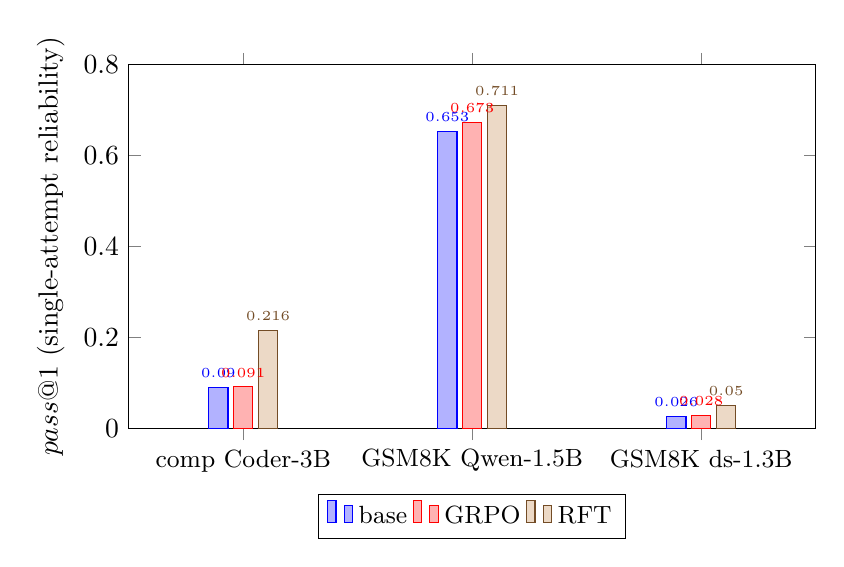
\begin{tikzpicture}
\begin{axis}[
  width=0.85\textwidth, height=6.2cm,
  ybar, bar width=7pt,
  ymin=0, ymax=0.8,
  ylabel={$\text{pass}@1$ (single-attempt reliability)},
  symbolic x coords={comp Coder-3B, GSM8K Qwen-1.5B, GSM8K ds-1.3B},
  xtick=data, x tick label style={font=\small},
  legend style={at={(0.5,-0.18)},anchor=north,legend columns=4,font=\small},
  enlarge x limits=0.25,
  nodes near coords, nodes near coords style={font=\tiny},
  every node near coord/.append style={/pgf/number format/fixed,/pgf/number format/precision=3},
]
\addplot coordinates {(comp Coder-3B,0.090) (GSM8K Qwen-1.5B,0.653) (GSM8K ds-1.3B,0.026)};
\addplot coordinates {(comp Coder-3B,0.091) (GSM8K Qwen-1.5B,0.673) (GSM8K ds-1.3B,0.028)};
\addplot coordinates {(comp Coder-3B,0.216) (GSM8K Qwen-1.5B,0.711) (GSM8K ds-1.3B,0.050)};
\legend{base, GRPO, RFT}
\end{axis}
\end{tikzpicture}
\caption{GRPO (orange) is visually indistinguishable from the base model (blue)
on single-attempt reliability, while RFT (green) acquires. Outcome RL rewards the
model's own verified successes yet fails to concentrate probability on them.}
\label{fig:ladder}
\end{figure}

\subsection*{2. A large reliability gap survives verified replay}

The second, and central, motivating fact is that \emph{even the winning recipe
leaves most of the achievable reliability on the table}. After RFT the model can
almost always \emph{produce} a correct solution within $k$ samples (high
coverage), yet a single sample is correct far less often (low $\text{pass}@1$).
Table~\ref{tab:gap} and Fig.~\ref{fig:gap} report this coverage$-$pass@1 gap
across nine cells spanning three model families (Qwen-Coder, Qwen, deepseek-coder),
sizes from $1.3$B to $7$B, and two domains. The gap is large and systematic
(often $0.20$--$0.50$), and it \emph{tracks the reliability headroom}: it is
widest where the base model is weak and shrinks toward zero only when the model
is already near-ceiling (GSM8K-3B, base $0.83$). In other words, the correct
solution is \emph{reachable} but the post-RFT model still spreads probability mass
across incorrect completions, so it will not be selected on the single attempt
that matters. Reachability is not reliability.

\begin{table}[htbp]
\centering
\caption{The reliability gap after decoupled verified replay: coverage
($\text{pass}@k$, $k{=}8$--$16$) greatly exceeds single-attempt reliability
($\text{pass}@1$) for the \emph{same} RFT checkpoint, across families, sizes, and
domains. The gap tracks headroom---large for weak/hard cells, near zero only at
ceiling. This residual is the opportunity our method targets.}
\label{tab:gap}
\begin{tabular}{llcccc}
\toprule
Domain & Model (difficulty) & base $\text{pass}@1$ & RFT $\text{pass}@1$ & RFT coverage & gap \\
\midrule
comp  & Coder-1.5B (mid)     & 0.053 & 0.246 & 0.745 & 0.499 \\
comp  & Coder-3B (hard)      & 0.090 & 0.216 & 0.610 & 0.394 \\
comp  & Coder-3B (vhard)     & 0.030 & 0.055 & 0.260 & 0.205 \\
comp  & deepseek-6.7B (mid)  & 0.268 & 0.361 & 0.805 & 0.444 \\
comp  & Qwen-7B (mid)        & 0.383 & 0.544 & 0.865 & 0.321 \\
comp  & Coder-7B (mid)       & 0.448 & 0.667 & 0.870 & 0.203 \\
GSM8K & Qwen-1.5B            & 0.653 & 0.711 & 0.918 & 0.207 \\
GSM8K & Qwen-3B (ceiling)    & 0.832 & 0.847 & 0.950 & 0.103 \\
\bottomrule
\end{tabular}
\end{table}

\begin{figure}[htbp]
\centering
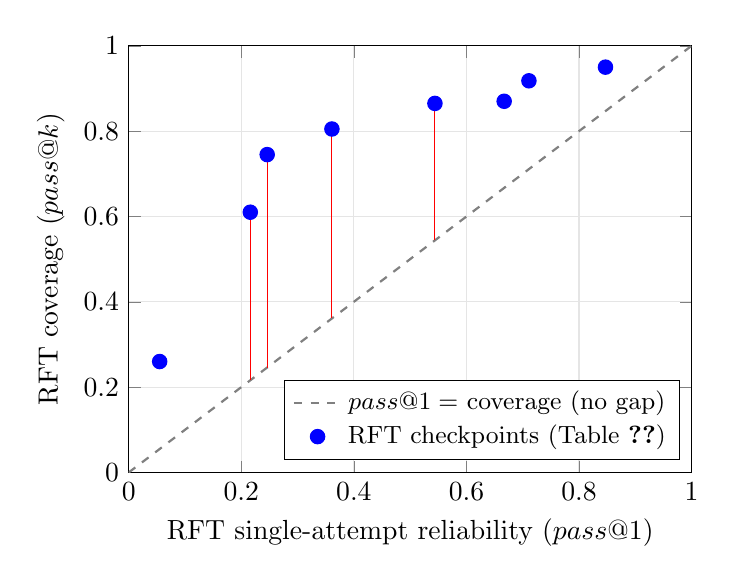
\begin{tikzpicture}
\begin{axis}[
  width=0.72\textwidth, height=7.0cm,
  xlabel={RFT single-attempt reliability ($\text{pass}@1$)},
  ylabel={RFT coverage ($\text{pass}@k$)},
  xmin=0, xmax=1, ymin=0, ymax=1,
  legend style={at={(0.98,0.03)},anchor=south east,font=\small},
  grid=both, grid style={gray!20},
]
% diagonal: reliability == coverage (the no-gap line)
\addplot[dashed, gray, thick, domain=0:1] {x};
\addlegendentry{$\text{pass}@1=$ coverage (no gap)}
% each point: (pass@1, coverage) for RFT
\addplot[only marks, mark=*, mark size=2.6pt, blue] coordinates {
  (0.246,0.745) (0.216,0.610) (0.055,0.260) (0.361,0.805)
  (0.544,0.865) (0.667,0.870) (0.711,0.918) (0.847,0.950)
};
\addlegendentry{RFT checkpoints (Table~\ref{tab:gap})}
% vertical gap segments
\addplot[red, thin] coordinates {(0.246,0.246) (0.246,0.745)};
\addplot[red, thin] coordinates {(0.216,0.216) (0.216,0.610)};
\addplot[red, thin] coordinates {(0.361,0.361) (0.361,0.805)};
\addplot[red, thin] coordinates {(0.544,0.544) (0.544,0.865)};
\end{axis}
\end{tikzpicture}
\caption{Every RFT checkpoint sits far \emph{above} the no-gap diagonal: the model
can reach a correct solution (high coverage, $y$) but rarely selects it on one
attempt (low $\text{pass}@1$, $x$). Red segments show the reliability gap. Verified
replay maximises \emph{coverage}; it does not close \emph{selection}.}
\label{fig:gap}
\end{figure}

\subsection*{3. The gap has a mechanistic cause: existing training does not
suppress verified-incorrect modes}

Why does verified replay stop short? We answer this mechanistically by
teacher-forcing each checkpoint over the \emph{same} held-out set of the model's
own verified-correct ($y^{+}$) and verified-incorrect ($y^{-}$) samples and
measuring the average per-token log-probability of each, together with the
correct-vs-incorrect \emph{logit margin} $m=\log\pi_\theta(y^{+})-\log\pi_\theta(y^{-})$
(Table~\ref{tab:margin}, Fig.~\ref{fig:margin}). Two clean signatures emerge.
First, \textbf{GRPO does not move the margin at all}: its $\log\pi(y^{+})$,
$\log\pi(y^{-})$, and $m$ are identical to the base model---the distributional
face of its $\approx\!0$ $\text{pass}@1$ gain, and consistent with the fact that
on-policy signal only reaches prompts the model already solves. Second,
\textbf{RFT is mode-covering}: it raises the log-probability of the correct
solution ($-0.110\!\to\!-0.092$) but raises the log-probability of the
\emph{incorrect} solution by essentially the same amount ($-0.139\!\to\!-0.119$),
so the margin barely changes ($0.029\!\to\!0.027$). Positive-only imitation lifts
correct \emph{and} incorrect modes together; it structurally cannot down-weight
the verified-wrong completions that steal single-attempt mass. This is precisely
why the reliability gap in \S2 persists: neither dominant recipe touches the
\emph{selection} axis---the reallocation of probability from verified-incorrect to
verified-correct on the same prompt.

\paragraph{Measurement protocol (rigor).} All log-probabilities are computed by
teacher-forcing each checkpoint on the \emph{identical} set of held-out verified
pairs (evaluation-disjoint from every training prompt), so the base/GRPO/RFT
numbers are strictly comparable and reflect the trained policies, not sampling
variation; decoding is frozen and the pairs are the model's own
verifier-labelled samples. The finding is not a single-model artifact: an
\emph{independent} per-prompt reliability-distribution analysis on a different
family and domain (Coder-3B, \textsc{CompDAG}; Fig.~\ref{fig:reldist}) reproduces
it---on-policy RL leaves $\approx\!79\%$ of prompts in the near-never-solved
region and verified replay rescues only a fraction, none by suppressing incorrect
modes---and the per-cell margin generalises across sizes and domains
(quantified in \S5.7). Two complementary measurements (per-token margin and
per-prompt reliability mass), two families, two domains: the mechanistic diagnosis
that motivates our method is robust, not anecdotal.

\begin{table}[htbp]
\centering
\caption{Mechanistic origin of the reliability gap (GSM8K, Qwen-1.5B; mean
per-token $\log\pi$ over 602 held-out verified pairs). GRPO leaves the margin at
the base value; RFT lifts correct \emph{and} incorrect log-probability together,
so the correct-vs-incorrect margin does not widen. No existing recipe suppresses
the verified-incorrect mode.}
\label{tab:margin}
\begin{tabular}{lccc}
\toprule
Stage & $\log\pi(y^{+})$ & $\log\pi(y^{-})$ & margin $m$ \\
\midrule
base  & $-0.110$ & $-0.139$ & 0.029 \\
GRPO  & $-0.109$ & $-0.139$ & 0.029 \\
RFT   & $-0.092$ & $-0.119$ & 0.027 \\
\bottomrule
\end{tabular}
\end{table}

\begin{figure}[htbp]
\centering
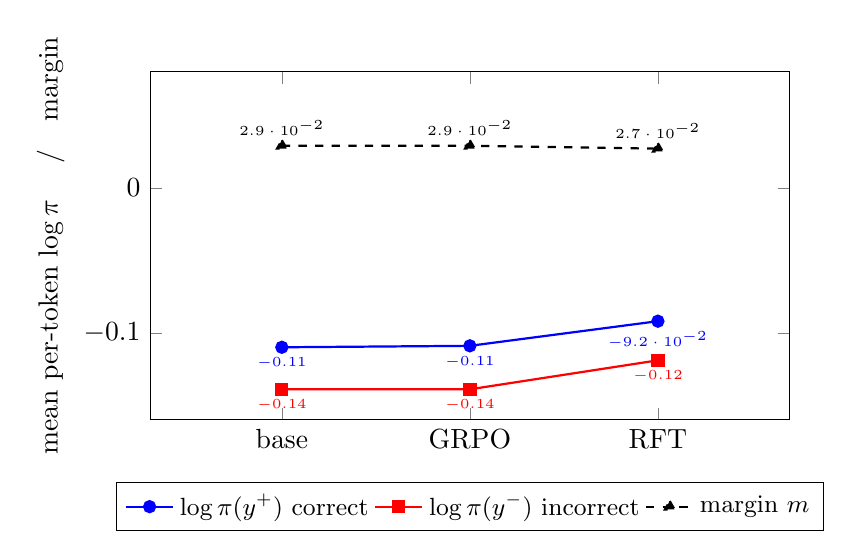
\begin{tikzpicture}
\begin{axis}[
  width=0.8\textwidth, height=6.0cm,
  ymin=-0.16, ymax=0.08,
  ylabel={mean per-token $\log\pi$ \quad/\quad margin},
  symbolic x coords={base, GRPO, RFT},
  xtick=data,
  legend style={at={(0.5,-0.18)},anchor=north,legend columns=3,font=\small},
  enlarge x limits=0.35,
  nodes near coords, nodes near coords style={font=\tiny},
]
\addplot[mark=*,blue,thick]   coordinates {(base,-0.110) (GRPO,-0.109) (RFT,-0.092)};
\addplot[mark=square*,red,thick] coordinates {(base,-0.139) (GRPO,-0.139) (RFT,-0.119)};
\addplot[mark=triangle*,black,thick,dashed] coordinates {(base,0.029) (GRPO,0.029) (RFT,0.027)};
\legend{$\log\pi(y^{+})$ correct, $\log\pi(y^{-})$ incorrect, margin $m$}
\end{axis}
\end{tikzpicture}
\caption{GRPO tracks the base model exactly (no movement). RFT raises the correct
\emph{and} incorrect log-probabilities in lock-step, so the margin (black dashed)
stays flat. The verified-incorrect mode is never suppressed---leaving the
selection axis, and hence single-attempt reliability, unaddressed.}
\label{fig:margin}
\end{figure}

\subsection*{The opportunity}

These three facts define the gap our work targets. (i) On-policy outcome RL
acquires almost no single-attempt reliability (Table~\ref{tab:ladder}); (ii) even
the best recipe, decoupled verified replay, leaves a large coverage$-$pass@1 gap
that scales with headroom (Table~\ref{tab:gap}); and (iii) the mechanistic reason
is that both recipes fail to suppress the verified-incorrect modes---they optimise
\emph{coverage} (reachability) and leave \emph{selection} (reliability) untouched
(Table~\ref{tab:margin}). Existing preference methods use verifier-labelled pairs
for alignment~\cite{rafailov2023dpo,hosseini2024vstar,yuan2024selfreward} but have
not been framed against, or evaluated on, this post-replay reliability residual.
This motivates the theory and methodology developed next: a \emph{decoupled,
verified-preference} objective that directly reallocates probability mass from
verified-incorrect to verified-correct solutions the model can already reach,
targeting the single axis---selection---that positive-only imitation and
on-policy reward provably leave open.
